\documentclass[11pt,letterpaper]{article}

% ============================================================================
% PACKAGES
% ============================================================================
\usepackage[utf8]{inputenc}
\usepackage[T1]{fontenc}
\usepackage{helvet}
\renewcommand{\familydefault}{\sfdefault}
\usepackage[margin=0.5in, top=0.5in, bottom=0.5in]{geometry}
\usepackage{xcolor}
\usepackage{tikz}
\usepackage{tcolorbox}
\usepackage{multicol}
\usepackage{enumitem}
\usepackage{parskip}
\usepackage{hyperref}

\usetikzlibrary{shapes.geometric, arrows.meta, positioning, calc, backgrounds, fit, decorations.pathreplacing}

% ============================================================================
% COLOR DEFINITIONS
% ============================================================================
\definecolor{humangate}{HTML}{27AE60}       % Green - Human gates
\definecolor{agentwork}{HTML}{3498DB}       % Blue - Agent work
\definecolor{reviewloop}{HTML}{9B59B6}      % Purple - Review/feedback
\definecolor{kanban}{HTML}{E67E22}          % Orange - Kanban states
\definecolor{darktext}{HTML}{2C3E50}        % Dark text
\definecolor{lightbg}{HTML}{F5F6F7}         % Light background
\definecolor{claude}{HTML}{CC785C}          % Claude orange-brown
\definecolor{gemini}{HTML}{4285F4}          % Gemini blue
\definecolor{codex}{HTML}{10A37F}           % OpenAI green

% ============================================================================
% DOCUMENT
% ============================================================================
\pagestyle{empty}
\setlength{\parskip}{0.3em}
\setlist{nosep, leftmargin=1.2em, itemsep=0.2em}

\begin{document}

% Header
\noindent
\begin{minipage}[t]{0.7\textwidth}
\textcolor{darktext}{\LARGE\textbf{AI-Assisted Development Workflow}}\\[0.2em]
\textcolor{darktext!70}{Human oversight with automated agent feedback loops}
\end{minipage}%
\hfill
\begin{minipage}[t]{0.25\textwidth}
\raggedleft
\textcolor{darktext!50}{\small Board-Centric Workflow v1.0}
\end{minipage}

\vspace{0.4em}
\hrule height 0.5pt
\vspace{0.6em}

% Main workflow diagram
\begin{center}
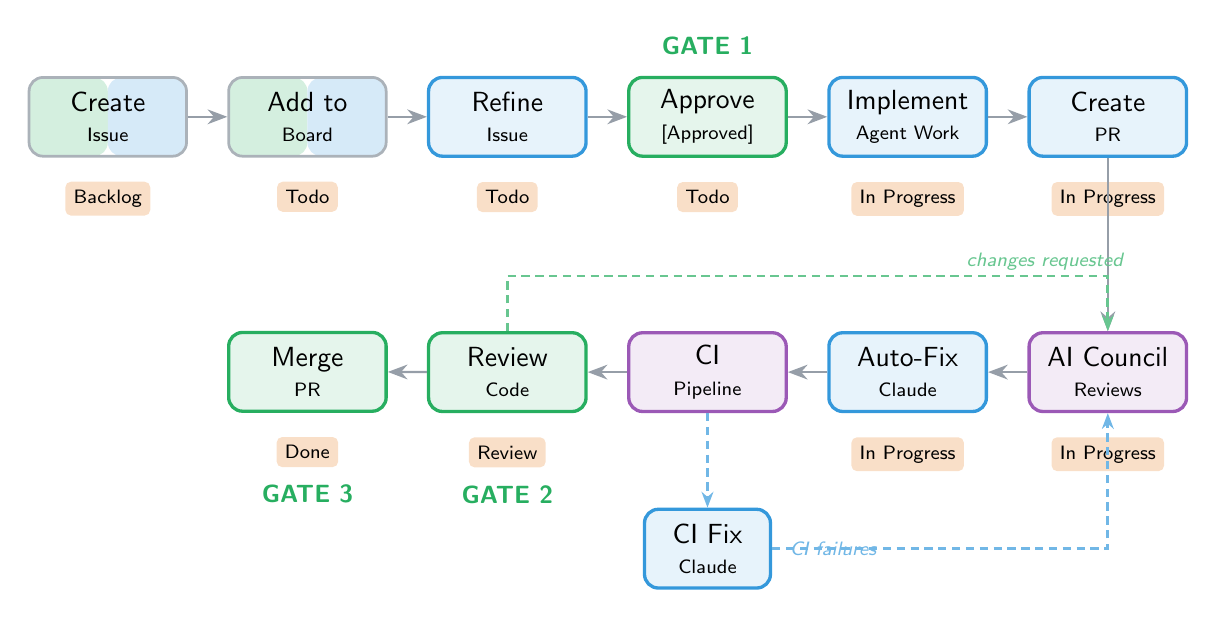
\begin{tikzpicture}[
  node distance=0.7cm and 0.5cm,
  every node/.style={font=\sffamily},
  stage/.style={rectangle, rounded corners=5pt, minimum height=1cm, minimum width=2cm, align=center, line width=1.2pt},
  human/.style={stage, draw=humangate, fill=humangate!12},
  agent/.style={stage, draw=agentwork, fill=agentwork!12},
  review/.style={stage, draw=reviewloop, fill=reviewloop!12},
  kanban/.style={rectangle, rounded corners=2pt, fill=kanban!25, font=\scriptsize\sffamily, inner sep=3pt},
  arrow/.style={-{Stealth[length=2.5mm]}, thick, color=darktext!50},
  looparrow/.style={-{Stealth[length=2mm]}, line width=1pt, color=reviewloop!80, densely dashed}
]

% === ROW 1: Forward Path (Left to Right) ===
% Hybrid style: half green (human), half blue (agent)
\node[stage, draw=darktext!40, line width=1pt,
      path picture={
        \fill[humangate!20] (path picture bounding box.north west) rectangle (path picture bounding box.south);
        \fill[agentwork!20] (path picture bounding box.north) rectangle (path picture bounding box.south east);
      }] (issue) {Create\\[-0.1em]{\scriptsize Issue}};

% Mixed human+agent node for board (half/half)
\node[stage, right=of issue, draw=darktext!40, line width=1pt,
      path picture={
        \fill[humangate!20] (path picture bounding box.north west) rectangle (path picture bounding box.south);
        \fill[agentwork!20] (path picture bounding box.north) rectangle (path picture bounding box.south east);
      }] (triage) {Add to\\[-0.1em]{\scriptsize Board}};

\node[agent, right=of triage] (refine) {Refine\\[-0.1em]{\scriptsize Issue}};
\node[human, right=of refine] (approve) {Approve\\[-0.1em]{\scriptsize [Approved]}};
\node[agent, right=of approve] (implement) {Implement\\[-0.1em]{\scriptsize Agent Work}};
\node[agent, right=of implement] (createpr) {Create\\[-0.1em]{\scriptsize PR}};

% Arrows
\draw[arrow] (issue) -- (triage);
\draw[arrow] (triage) -- (refine);
\draw[arrow] (refine) -- (approve);
\draw[arrow] (approve) -- (implement);
\draw[arrow] (implement) -- (createpr);

% Gate label
\node[above=0.15cm of approve, font=\small\bfseries\color{humangate}] {GATE 1};

% Kanban below row 1
\node[kanban, below=0.3cm of issue] {Backlog};
\node[kanban, below=0.3cm of triage] {Todo};
\node[kanban, below=0.3cm of refine] {Todo};
\node[kanban, below=0.3cm of approve] {Todo};
\node[kanban, below=0.3cm of implement] {In Progress};
\node[kanban, below=0.3cm of createpr] {In Progress};

% === ROW 2: Review Path (Right to Left) ===
\node[review, below=2.2cm of createpr] (council) {AI Council\\[-0.1em]{\scriptsize Reviews}};
\node[agent, below=2.2cm of implement] (autofix) {Auto-Fix\\[-0.1em]{\scriptsize Claude}};
\node[review, below=2.2cm of approve] (ci) {CI\\[-0.1em]{\scriptsize Pipeline}};
\node[human, below=2.2cm of refine] (humanrev) {Review\\[-0.1em]{\scriptsize Code}};
\node[human, below=2.2cm of triage] (merge) {Merge\\[-0.1em]{\scriptsize PR}};

% CI Failure Auto-Fix box (below CI Pipeline)
\node[agent, below=1.2cm of ci, minimum width=1.6cm] (cifix) {CI Fix\\[-0.1em]{\scriptsize Claude}};

% Main flow arrows
\draw[arrow] (createpr) -- (council);
\draw[arrow] (council) -- (autofix);
\draw[arrow] (autofix) -- (ci);
\draw[arrow] (ci) -- (humanrev);
\draw[arrow] (humanrev) -- (merge);

% Kanban below row 2 (shifted for cifix)
\node[kanban, below=0.3cm of council] {In Progress};
\node[kanban, below=0.3cm of autofix] {In Progress};
\node[kanban, below=0.3cm of humanrev] {Review};
\node[kanban, below=0.3cm of merge] {Done};

% Gate labels row 2 (below kanban)
\node[below=0.8cm of humanrev, font=\small\bfseries\color{humangate}] {GATE 2};
\node[below=0.8cm of merge, font=\small\bfseries\color{humangate}] {GATE 3};

% === FEEDBACK LOOPS ===
% Human review can request changes -> back to council (above, higher than purple)
\draw[looparrow, humangate!70] (humanrev.north) -- ++(0,0.7) -| (council.north);

% CI failure loop (down to CI Fix, back to AI Council)
\draw[looparrow, agentwork!70] (ci.south) -- (cifix.north);
\draw[looparrow, agentwork!70] (cifix.east) -| (council.south);

% Loop labels
\node[above=0.65cm of council, font=\scriptsize\color{humangate!70}\itshape, xshift=-0.8cm] {changes requested};
\node[right=0.1cm of cifix, font=\scriptsize\color{agentwork!70}\itshape] {CI failures};

\end{tikzpicture}
\end{center}

\vspace{0.3em}

% Legend bar
\begin{center}
\fcolorbox{lightbg}{lightbg}{%
\begin{tabular}{@{}c@{\hspace{0.8em}}c@{\hspace{0.8em}}c@{\hspace{0.8em}}c@{\hspace{0.8em}}c@{}}
\tikz\fill[humangate!35, rounded corners=2pt] (0,0) rectangle (0.4,0.25); \textsf{\small Human} &
\tikz\fill[agentwork!35, rounded corners=2pt] (0,0) rectangle (0.4,0.25); \textsf{\small Agent} &
\tikz{\fill[humangate!25, rounded corners=2pt] (0,0) rectangle (0.2,0.25); \fill[agentwork!25, rounded corners=2pt] (0.2,0) rectangle (0.4,0.25);} \textsf{\small Hybrid} &
\tikz\fill[reviewloop!35, rounded corners=2pt] (0,0) rectangle (0.4,0.25); \textsf{\small Review} &
\tikz\fill[kanban!40, rounded corners=2pt] (0,0) rectangle (0.4,0.25); \textsf{\small Kanban}
\end{tabular}%
}
\end{center}

\vspace{0.5em}

% Three-column content
\begin{multicols}{3}

% Column 1: Human Gates
\textcolor{humangate}{\Large\textbf{Human Gates}}
\vspace{0.3em}

\textbf{Three checkpoints} for oversight:

\begin{enumerate}[label=\textbf{\arabic*.}, leftmargin=1.5em, itemsep=0.3em]
  \item \textbf{Approve Work}\\
        {\small \texttt{[Approved]} triggers agent}
  \item \textbf{Code Review}\\
        {\small Can request changes $\rightarrow$ loops back}
  \item \textbf{Merge PR}\\
        {\small Final merge decision}
\end{enumerate}

\vspace{0.4em}

{\small Both humans and agents can add issues to the board.}

\vspace{0.6em}
\textcolor{reviewloop}{\Large\textbf{Agent Council}}
\vspace{0.3em}

Three AI review perspectives:

\begin{itemize}[leftmargin=1.2em, itemsep=0.3em]
  \item \textcolor{gemini}{\textbf{Gemini}} -- Security \& architecture
  \item \textcolor{codex}{\textbf{Codex}} -- Code patterns \& quality
  \item \textcolor{claude}{\textbf{Claude}} -- Implementation \& fixes
\end{itemize}

\vspace{0.3em}
{\small Maintainer feedback always takes priority over AI suggestions.}

\columnbreak

% Column 2: Feedback Loops
\textcolor{agentwork}{\Large\textbf{Feedback Loops}}
\vspace{0.3em}

Two automated loops minimize human round-trips:

\vspace{0.5em}
\begin{tcolorbox}[colback=agentwork!10, colframe=agentwork!60, boxrule=0.8pt, arc=3pt, left=6pt, right=6pt, top=5pt, bottom=5pt, title={\small\textbf{Loop 1: Review Response}}, fonttitle=\sffamily\bfseries, coltitle=white, colbacktitle=agentwork!70]
{\small
Gemini/Codex posts review\\[0.2em]
$\rightarrow$ Claude auto-fixes issues\\[0.2em]
$\rightarrow$ Push triggers re-review}
\end{tcolorbox}

\vspace{0.4em}

\begin{tcolorbox}[colback=reviewloop!10, colframe=reviewloop!60, boxrule=0.8pt, arc=3pt, left=6pt, right=6pt, top=5pt, bottom=5pt, title={\small\textbf{Loop 2: CI Failures}}, fonttitle=\sffamily\bfseries, coltitle=white, colbacktitle=reviewloop!70]
{\small
Format or lint check fails\\[0.2em]
$\rightarrow$ Auto-fix applied\\[0.2em]
$\rightarrow$ Push triggers re-run}
\end{tcolorbox}

\vspace{0.5em}
\textbf{Safety mechanisms:}
\begin{itemize}[leftmargin=1.2em, itemsep=0.2em]
  \item Max 5 iterations per PR
  \item \texttt{[AI-AUTO-FIX]} commit markers
  \item Skips reviews on agent commits
\end{itemize}

\columnbreak

% Column 3: Kanban + Key Insight
\textcolor{kanban}{\Large\textbf{Kanban Flow}}
\vspace{0.3em}

Board status tracks workflow progress:

\vspace{0.5em}
\begin{center}
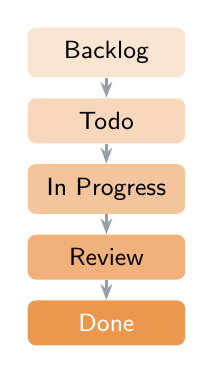
\begin{tikzpicture}[node distance=0.25cm, every node/.style={font=\small\sffamily}]
  \node[fill=kanban!20, rounded corners=3pt, inner sep=5pt, minimum width=2cm] (b) {Backlog};
  \node[fill=kanban!30, rounded corners=3pt, inner sep=5pt, minimum width=2cm, below=of b] (t) {Todo};
  \node[fill=kanban!45, rounded corners=3pt, inner sep=5pt, minimum width=2cm, below=of t] (p) {In Progress};
  \node[fill=kanban!60, rounded corners=3pt, inner sep=5pt, minimum width=2cm, below=of p] (r) {Review};
  \node[fill=kanban!80, rounded corners=3pt, inner sep=5pt, minimum width=2cm, below=of r, text=white] (d) {Done};
  \draw[-{Stealth[length=2mm]}, darktext!50, thick] (b) -- (t);
  \draw[-{Stealth[length=2mm]}, darktext!50, thick] (t) -- (p);
  \draw[-{Stealth[length=2mm]}, darktext!50, thick] (p) -- (r);
  \draw[-{Stealth[length=2mm]}, darktext!50, thick] (r) -- (d);
\end{tikzpicture}
\end{center}

\vspace{0.4em}
{\small Issues move through stages automatically as agents work. \textbf{Blocked} state available for dependency management.}

\vspace{0.6em}

\begin{tcolorbox}[colback=darktext!8, colframe=darktext!40, boxrule=0.8pt, arc=3pt, left=6pt, right=6pt, top=6pt, bottom=6pt]
\textbf{\large Key Insight}\\[0.3em]
\textcolor{humangate}{\textbf{Humans}} decide \textbf{what} to work on and \textbf{when} to merge.\\[0.3em]
\textcolor{agentwork}{\textbf{Agents}} handle \textbf{how} with automated quality loops.
\end{tcolorbox}

\end{multicols}

\end{document}
